\documentclass{article}
\usepackage{graphicx}
\usepackage{caption}
\usepackage{geometry}
\geometry{a4paper, margin=1in}

\title{Rapport de Statistiques des Parties}
\author{Application de Jeu}
\date{\today}

\begin{document}

\maketitle

\section*{Introduction}
Ce rapport présente les statistiques des parties jouées, incluant le nombre de manches réussies, les valeurs ayant causé des échecs, et le temps de réaction moyen.

\section*{Nombre de Manches Réussies par Partie}
\begin{figure}[h!]
    \centering
    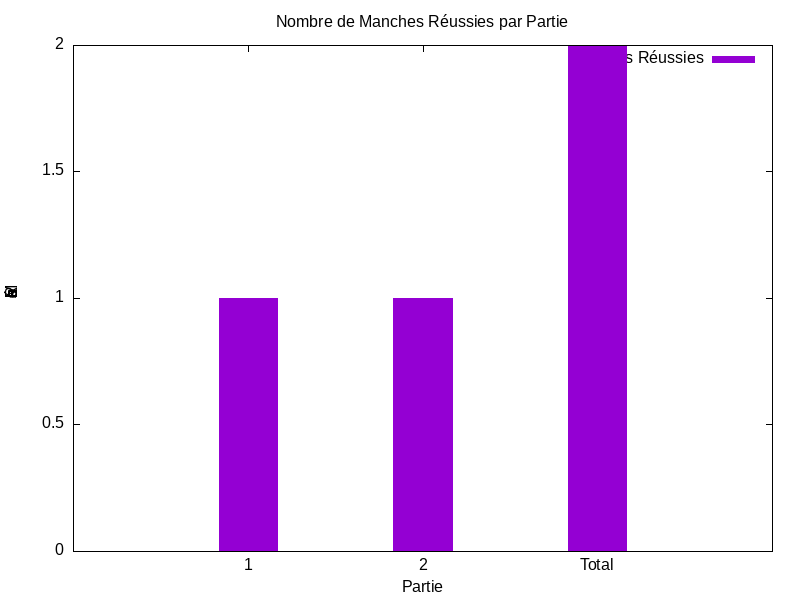
\includegraphics[width=0.8\textwidth]{manches_reussies.png}
    \caption{Histogramme du nombre de manches réussies par partie}
\end{figure}

\section*{Valeur ayant Causé un Échec par Partie}
\begin{figure}[h!]
    \centering
    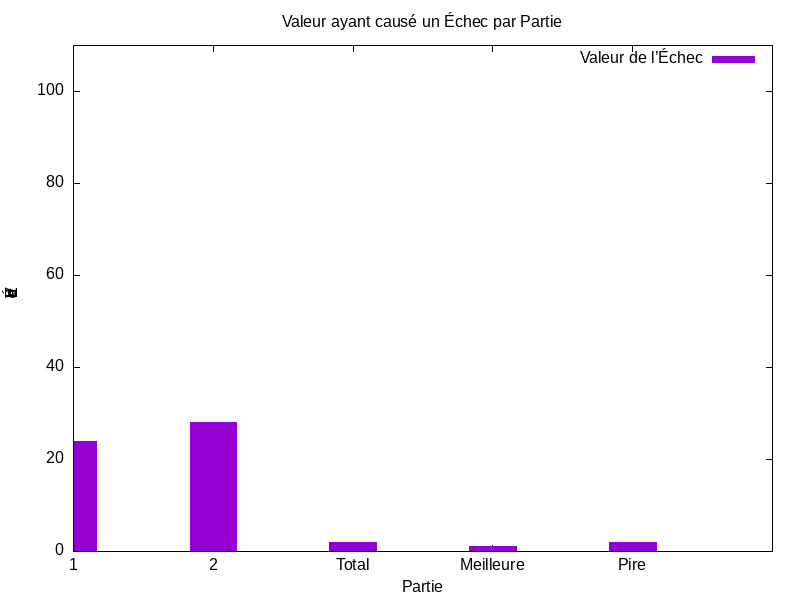
\includegraphics[width=0.8\textwidth]{valeur_echec.png}
    \caption{Histogramme des valeurs ayant causé un échec par partie}
\end{figure}

\section*{Temps de Réaction Moyen par Partie}
\begin{figure}[h!]
    \centering
    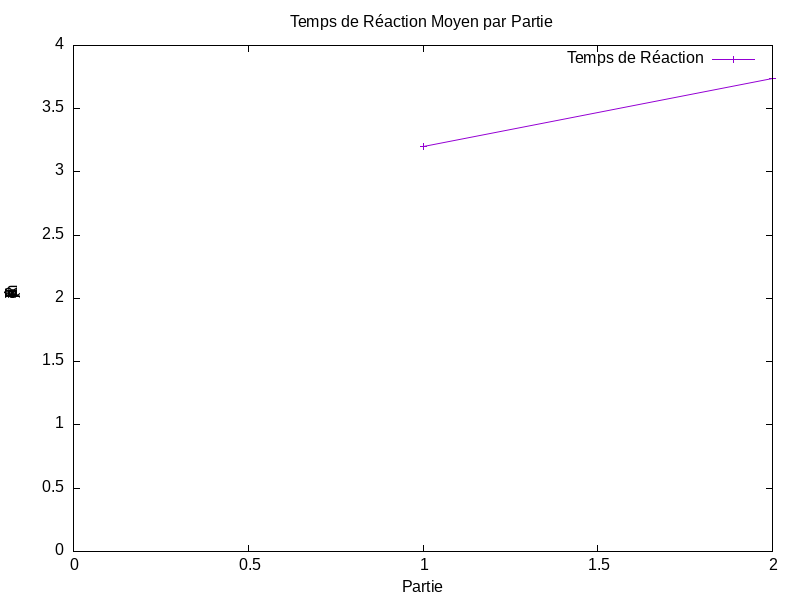
\includegraphics[width=0.8\textwidth]{temps_reaction.png}
    \caption{Graphique en ligne du temps de réaction moyen par partie}
\end{figure}

\section*{Tableau des Statistiques}
\begin{table}[ht!]
\centering
\begin{table}[ht]
\centering
\begin{tabular}{|l|l|l|l|}
\hline
Partie & Manches Reussies & Valeur de l Echec & Temps de Reaction (secondes) \\ \hline
1 1 24 3.2050 &  &  &  \\ \hline
2 1 28 3.7400 &  &  &  \\ \hline
Total & 2 & 2 & - \\ \hline
Meilleure Partie & 1 & - & 3.2050 \\ \hline
Pire Partie & 2 & - & 3.7400 \\ \hline
Temps de Réaction Moyen & - & - & 0.0003 \\ \hline
\end{tabular}
\caption{Tableau des statistiques des parties}
\end{table}
 % Inclut le tableau LaTeX généré
\caption{Tableau des statistiques des parties}
\end{table}

\end{document}
\section*{Résumé des Statistiques}
\begin{itemize}
\item Total des Manches Réussies : 
\item Nombre total de Valeurs Loupées : 
\item Meilleure Partie : Partie  avec un temps de réaction de  secondes
\item Pire Partie : Partie  avec un temps de réaction de  secondes
\end{itemize}
\section*{Tableau des Statistiques}
\begin{table}[ht!]
\centering
\begin{table}[ht]
\centering
\begin{tabular}{|l|l|l|l|}
\hline
Partie & Manches Reussies & Valeur de l Echec & Temps de Reaction (secondes) \\ \hline
1 1 24 3.2050 &  &  &  \\ \hline
2 1 28 3.7400 &  &  &  \\ \hline
Total & 2 & 2 & - \\ \hline
Meilleure Partie & 1 & - & 3.2050 \\ \hline
Pire Partie & 2 & - & 3.7400 \\ \hline
Temps de Réaction Moyen & - & - & 0.0003 \\ \hline
\end{tabular}
\caption{Tableau des statistiques des parties}
\end{table}

\caption{Tableau des statistiques des parties}
\end{table}
\section*{Résumé des Statistiques}
\begin{itemize}
\item Total des Manches Réussies : 
\item Nombre total de Valeurs Loupées : 
\item Meilleure Partie : Partie  avec un temps de réaction de  secondes
\item Pire Partie : Partie  avec un temps de réaction de  secondes
\end{itemize}
\section*{Tableau des Statistiques}
\begin{table}[ht]
\centering
\begin{tabular}{|l|l|l|l|}
\hline
Partie & Manches Reussies & Valeur de l Echec & Temps de Reaction (secondes) \\ \hline
1 1 24 3.2050 &  &  &  \\ \hline
2 1 28 3.7400 &  &  &  \\ \hline
Total & 2 & 2 & - \\ \hline
Meilleure Partie & 1 & - & 3.2050 \\ \hline
Pire Partie & 2 & - & 3.7400 \\ \hline
Temps de Réaction Moyen & - & - & 0.0003 \\ \hline
\end{tabular}
\caption{Tableau des statistiques des parties}
\end{table}

\section*{Résumé des Statistiques}
\begin{itemize}
\item Total des Manches Réussies : 
\item Nombre total de Valeurs Loupées : 
\item Meilleure Partie : Partie  avec un temps de réaction de  secondes
\item Pire Partie : Partie  avec un temps de réaction de  secondes
\end{itemize}
\section*{Tableau des Statistiques}
\begin{table}[ht]
\centering
\begin{tabular}{|l|l|l|l|}
\hline
Partie & Manches Reussies & Valeur de l Echec & Temps de Reaction (secondes) \\ \hline
1 1 24 3.2050 &  &  &  \\ \hline
2 1 28 3.7400 &  &  &  \\ \hline
Total & 2 & 2 & - \\ \hline
Meilleure Partie & 1 & - & 3.2050 \\ \hline
Pire Partie & 2 & - & 3.7400 \\ \hline
Temps de Réaction Moyen & - & - & 0.0003 \\ \hline
\end{tabular}
\caption{Tableau des statistiques des parties}
\end{table}

\section*{Résumé des Statistiques}
\begin{itemize}
\item Total des Manches Réussies : 
\item Nombre total de Valeurs Loupées : 
\item Meilleure Partie : Partie  avec un temps de réaction de  secondes
\item Pire Partie : Partie  avec un temps de réaction de  secondes
\end{itemize}
\section*{Tableau des Statistiques}
\begin{table}[ht]
\centering
\begin{tabular}{|l|l|l|l|}
\hline
Partie & Manches Reussies & Valeur de l Echec & Temps de Reaction (secondes) \\ \hline
1 1 24 3.2050 &  &  &  \\ \hline
2 1 28 3.7400 &  &  &  \\ \hline
Total & 2 & 2 & - \\ \hline
Meilleure Partie & 1 & - & 3.2050 \\ \hline
Pire Partie & 2 & - & 3.7400 \\ \hline
Temps de Réaction Moyen & - & - & 0.0003 \\ \hline
\end{tabular}
\caption{Tableau des statistiques des parties}
\end{table}

\section*{Résumé des Statistiques}
\begin{itemize}
\item Total des Manches Réussies : 
\item Nombre total de Valeurs Loupées : 
\item Meilleure Partie : Partie  avec un temps de réaction de  secondes
\item Pire Partie : Partie  avec un temps de réaction de  secondes
\end{itemize}
\section*{Tableau des Statistiques}
\begin{table}[ht]
\centering
\begin{tabular}{|l|l|l|l|}
\hline
Partie & Manches Reussies & Valeur de l Echec & Temps de Reaction (secondes) \\ \hline
1 1 24 3.2050 &  &  &  \\ \hline
2 1 28 3.7400 &  &  &  \\ \hline
Total & 2 & 2 & - \\ \hline
Meilleure Partie & 1 & - & 3.2050 \\ \hline
Pire Partie & 2 & - & 3.7400 \\ \hline
Temps de Réaction Moyen & - & - & 0.0003 \\ \hline
\end{tabular}
\caption{Tableau des statistiques des parties}
\end{table}

\section*{Résumé des Statistiques}
\begin{itemize}
\item Total des Manches Réussies : 
\item Nombre total de Valeurs Loupées : 
\item Meilleure Partie : Partie  avec un temps de réaction de  secondes
\item Pire Partie : Partie  avec un temps de réaction de  secondes
\end{itemize}
\section*{Tableau des Statistiques}
\begin{table}[ht]
\centering
\begin{tabular}{|l|l|l|l|}
\hline
Partie & Manches Reussies & Valeur de l Echec & Temps de Reaction (secondes) \\ \hline
1 1 24 3.2050 &  &  &  \\ \hline
2 1 28 3.7400 &  &  &  \\ \hline
Total & 2 & 2 & - \\ \hline
Meilleure Partie & 1 & - & 3.2050 \\ \hline
Pire Partie & 2 & - & 3.7400 \\ \hline
Temps de Réaction Moyen & - & - & 0.0003 \\ \hline
\end{tabular}
\caption{Tableau des statistiques des parties}
\end{table}

\section*{Résumé des Statistiques}
\begin{itemize}
\item Total des Manches Réussies : 
\item Nombre total de Valeurs Loupées : 
\item Meilleure Partie : Partie  avec un temps de réaction de  secondes
\item Pire Partie : Partie  avec un temps de réaction de  secondes
\end{itemize}
\section*{Tableau des Statistiques}
\begin{table}[ht]
\centering
\begin{tabular}{|l|l|l|l|}
\hline
Partie & Manches Reussies & Valeur de l Echec & Temps de Reaction (secondes) \\ \hline
1 1 24 3.2050 &  &  &  \\ \hline
2 1 28 3.7400 &  &  &  \\ \hline
Total & 2 & 2 & - \\ \hline
Meilleure Partie & 1 & - & 3.2050 \\ \hline
Pire Partie & 2 & - & 3.7400 \\ \hline
Temps de Réaction Moyen & - & - & 0.0003 \\ \hline
\end{tabular}
\caption{Tableau des statistiques des parties}
\end{table}

\section*{Résumé des Statistiques}
\begin{itemize}
\item Total des Manches Réussies : 
\item Nombre total de Valeurs Loupées : 
\item Meilleure Partie : Partie  avec un temps de réaction de  secondes
\item Pire Partie : Partie  avec un temps de réaction de  secondes
\end{itemize}
\section*{Tableau des Statistiques}
\begin{table}[ht]
\centering
\begin{tabular}{|l|l|l|l|}
\hline
Partie & Manches Reussies & Valeur de l Echec & Temps de Reaction (secondes) \\ \hline
1 1 24 3.2050 &  &  &  \\ \hline
2 1 28 3.7400 &  &  &  \\ \hline
Total & 2 & 2 & - \\ \hline
Meilleure Partie & 1 & - & 3.2050 \\ \hline
Pire Partie & 2 & - & 3.7400 \\ \hline
Temps de Réaction Moyen & - & - & 0.0003 \\ \hline
\end{tabular}
\caption{Tableau des statistiques des parties}
\end{table}

\section*{Résumé des Statistiques}
\begin{itemize}
\item Total des Manches Réussies : 
\item Nombre total de Valeurs Loupées : 
\item Meilleure Partie : Partie  avec un temps de réaction de  secondes
\item Pire Partie : Partie  avec un temps de réaction de  secondes
\end{itemize}
\section*{Tableau des Statistiques}
\begin{table}[ht]
\centering
\begin{tabular}{|l|l|l|l|}
\hline
Partie & Manches Reussies & Valeur de l Echec & Temps de Reaction (secondes) \\ \hline
1 1 24 3.2050 &  &  &  \\ \hline
2 1 28 3.7400 &  &  &  \\ \hline
Total & 2 & 2 & - \\ \hline
Meilleure Partie & 1 & - & 3.2050 \\ \hline
Pire Partie & 2 & - & 3.7400 \\ \hline
Temps de Réaction Moyen & - & - & 0.0003 \\ \hline
\end{tabular}
\caption{Tableau des statistiques des parties}
\end{table}

\section*{Résumé des Statistiques}
\begin{itemize}
\item Total des Manches Réussies : 
\item Nombre total de Valeurs Loupées : 
\item Meilleure Partie : Partie  avec un temps de réaction de  secondes
\item Pire Partie : Partie  avec un temps de réaction de  secondes
\end{itemize}
\section*{Tableau des Statistiques}
\begin{table}[ht]
\centering
\begin{tabular}{|l|l|l|l|}
\hline
Partie & Manches Reussies & Valeur de l Echec & Temps de Reaction (secondes) \\ \hline
1 1 24 3.2050 &  &  &  \\ \hline
2 1 28 3.7400 &  &  &  \\ \hline
Total & 2 & 2 & - \\ \hline
Meilleure Partie & 1 & - & 3.2050 \\ \hline
Pire Partie & 2 & - & 3.7400 \\ \hline
Temps de Réaction Moyen & - & - & 0.0003 \\ \hline
\end{tabular}
\caption{Tableau des statistiques des parties}
\end{table}

\section*{Résumé des Statistiques}
\begin{itemize}
\item Total des Manches Réussies : 
\item Nombre total de Valeurs Loupées : 
\item Meilleure Partie : Partie  avec un temps de réaction de  secondes
\item Pire Partie : Partie  avec un temps de réaction de  secondes
\end{itemize}
\section*{Tableau des Statistiques}
\begin{table}[ht]
\centering
\begin{tabular}{|l|l|l|l|}
\hline
Partie & Manches Reussies & Valeur de l Echec & Temps de Reaction (secondes) \\ \hline
1 1 24 3.2050 &  &  &  \\ \hline
2 1 28 3.7400 &  &  &  \\ \hline
Total & 2 & 2 & - \\ \hline
Meilleure Partie & 1 & - & 3.2050 \\ \hline
Pire Partie & 2 & - & 3.7400 \\ \hline
Temps de Réaction Moyen & - & - & 0.0003 \\ \hline
\end{tabular}
\caption{Tableau des statistiques des parties}
\end{table}

\section*{Résumé des Statistiques}
\begin{itemize}
\item Total des Manches Réussies : 
\item Nombre total de Valeurs Loupées : 
\item Meilleure Partie : Partie  avec un temps de réaction de  secondes
\item Pire Partie : Partie  avec un temps de réaction de  secondes
\end{itemize}
\section*{Tableau des Statistiques}
\begin{table}[ht]
\centering
\begin{tabular}{|l|l|l|l|}
\hline
Partie & Manches Reussies & Valeur de l Echec & Temps de Reaction (secondes) \\ \hline
1 1 24 3.2050 &  &  &  \\ \hline
2 1 28 3.7400 &  &  &  \\ \hline
Total & 2 & 2 & - \\ \hline
Meilleure Partie & 1 & - & 3.2050 \\ \hline
Pire Partie & 2 & - & 3.7400 \\ \hline
Temps de Réaction Moyen & - & - & 0.0003 \\ \hline
\end{tabular}
\caption{Tableau des statistiques des parties}
\end{table}

\section*{Résumé des Statistiques}
\begin{itemize}
\item Total des Manches Réussies : 
\item Nombre total de Valeurs Loupées : 
\item Meilleure Partie : Partie  avec un temps de réaction de  secondes
\item Pire Partie : Partie  avec un temps de réaction de  secondes
\end{itemize}
\section*{Tableau des Statistiques}
\begin{table}[ht]
\centering
\begin{tabular}{|l|l|l|l|}
\hline
Partie & Manches Reussies & Valeur de l Echec & Temps de Reaction (secondes) \\ \hline
1 1 24 3.2050 &  &  &  \\ \hline
2 1 28 3.7400 &  &  &  \\ \hline
Total & 2 & 2 & - \\ \hline
Meilleure Partie & 1 & - & 3.2050 \\ \hline
Pire Partie & 2 & - & 3.7400 \\ \hline
Temps de Réaction Moyen & - & - & 0.0003 \\ \hline
\end{tabular}
\caption{Tableau des statistiques des parties}
\end{table}

\section*{Résumé des Statistiques}
\begin{itemize}
\item Total des Manches Réussies : 
\item Nombre total de Valeurs Loupées : 
\item Meilleure Partie : Partie  avec un temps de réaction de  secondes
\item Pire Partie : Partie  avec un temps de réaction de  secondes
\end{itemize}
\section*{Tableau des Statistiques}
\begin{table}[ht]
\centering
\begin{tabular}{|l|l|l|l|}
\hline
Partie & Manches Reussies & Valeur de l Echec & Temps de Reaction (secondes) \\ \hline
1 1 24 3.2050 &  &  &  \\ \hline
2 1 28 3.7400 &  &  &  \\ \hline
Total & 2 & 2 & - \\ \hline
Meilleure Partie & 1 & - & 3.2050 \\ \hline
Pire Partie & 2 & - & 3.7400 \\ \hline
Temps de Réaction Moyen & - & - & 0.0003 \\ \hline
\end{tabular}
\caption{Tableau des statistiques des parties}
\end{table}

\section*{Résumé des Statistiques}
\begin{itemize}
\item Total des Manches Réussies : 
\item Nombre total de Valeurs Loupées : 
\item Meilleure Partie : Partie  avec un temps de réaction de  secondes
\item Pire Partie : Partie  avec un temps de réaction de  secondes
\end{itemize}
\section*{Tableau des Statistiques}
\begin{table}[ht]
\centering
\begin{tabular}{|l|l|l|l|}
\hline
Partie & Manches Reussies & Valeur de l Echec & Temps de Reaction (secondes) \\ \hline
1 1 24 3.2050 &  &  &  \\ \hline
2 1 28 3.7400 &  &  &  \\ \hline
Total & 2 & 2 & - \\ \hline
Meilleure Partie & 1 & - & 3.2050 \\ \hline
Pire Partie & 2 & - & 3.7400 \\ \hline
Temps de Réaction Moyen & - & - & 0.0003 \\ \hline
\end{tabular}
\caption{Tableau des statistiques des parties}
\end{table}

\section*{Résumé des Statistiques}
\begin{itemize}
\item Total des Manches Réussies : 
\item Nombre total de Valeurs Loupées : 
\item Meilleure Partie : Partie  avec un temps de réaction de  secondes
\item Pire Partie : Partie  avec un temps de réaction de  secondes
\end{itemize}
\section*{Tableau des Statistiques}
\begin{table}[ht]
\centering
\begin{tabular}{|l|l|l|l|}
\hline
Partie & Manches Reussies & Valeur de l Echec & Temps de Reaction (secondes) \\ \hline
1 1 24 3.2050 &  &  &  \\ \hline
2 1 28 3.7400 &  &  &  \\ \hline
Total & 2 & 2 & - \\ \hline
Meilleure Partie & 1 & - & 3.2050 \\ \hline
Pire Partie & 2 & - & 3.7400 \\ \hline
Temps de Réaction Moyen & - & - & 0.0003 \\ \hline
\end{tabular}
\caption{Tableau des statistiques des parties}
\end{table}

\section*{Résumé des Statistiques}
\begin{itemize}
\item Total des Manches Réussies : 
\item Nombre total de Valeurs Loupées : 
\item Meilleure Partie : Partie  avec un temps de réaction de  secondes
\item Pire Partie : Partie  avec un temps de réaction de  secondes
\end{itemize}
\section*{Tableau des Statistiques}
\begin{table}[ht]
\centering
\begin{tabular}{|l|l|l|l|}
\hline
Partie & Manches Reussies & Valeur de l Echec & Temps de Reaction (secondes) \\ \hline
1 1 24 3.2050 &  &  &  \\ \hline
2 1 28 3.7400 &  &  &  \\ \hline
Total & 2 & 2 & - \\ \hline
Meilleure Partie & 1 & - & 3.2050 \\ \hline
Pire Partie & 2 & - & 3.7400 \\ \hline
Temps de Réaction Moyen & - & - & 0.0003 \\ \hline
\end{tabular}
\caption{Tableau des statistiques des parties}
\end{table}

\section*{Résumé des Statistiques}
\begin{itemize}
\item Total des Manches Réussies : 
\item Nombre total de Valeurs Loupées : 
\item Meilleure Partie : Partie  avec un temps de réaction de  secondes
\item Pire Partie : Partie  avec un temps de réaction de  secondes
\end{itemize}
\section*{Tableau des Statistiques}
\begin{table}[ht]
\centering
\begin{tabular}{|l|l|l|l|}
\hline
Partie & Manches Reussies & Valeur de l Echec & Temps de Reaction (secondes) \\ \hline
1 1 24 3.2050 &  &  &  \\ \hline
2 1 28 3.7400 &  &  &  \\ \hline
Total & 2 & 2 & - \\ \hline
Meilleure Partie & 1 & - & 3.2050 \\ \hline
Pire Partie & 2 & - & 3.7400 \\ \hline
Temps de Réaction Moyen & - & - & 0.0003 \\ \hline
\end{tabular}
\caption{Tableau des statistiques des parties}
\end{table}

\section*{Résumé des Statistiques}
\begin{itemize}
\item Total des Manches Réussies : 
\item Nombre total de Valeurs Loupées : 
\item Meilleure Partie : Partie  avec un temps de réaction de  secondes
\item Pire Partie : Partie  avec un temps de réaction de  secondes
\end{itemize}
\section*{Tableau des Statistiques}
\begin{table}[ht]
\centering
\begin{tabular}{|l|l|l|l|}
\hline
Partie & Manches Reussies & Valeur de l Echec & Temps de Reaction (secondes) \\ \hline
1 1 24 3.2050 &  &  &  \\ \hline
2 1 28 3.7400 &  &  &  \\ \hline
Total & 2 & 2 & - \\ \hline
Meilleure Partie & 1 & - & 3.2050 \\ \hline
Pire Partie & 2 & - & 3.7400 \\ \hline
Temps de Réaction Moyen & - & - & 0.0003 \\ \hline
\end{tabular}
\caption{Tableau des statistiques des parties}
\end{table}

\section*{Résumé des Statistiques}
\begin{itemize}
\item Total des Manches Réussies : 
\item Nombre total de Valeurs Loupées : 
\item Meilleure Partie : Partie  avec un temps de réaction de  secondes
\item Pire Partie : Partie  avec un temps de réaction de  secondes
\end{itemize}
\section*{Tableau des Statistiques}
\begin{table}[ht]
\centering
\begin{tabular}{|l|l|l|l|}
\hline
Partie & Manches Reussies & Valeur de l Echec & Temps de Reaction (secondes) \\ \hline
1 1 24 3.2050 &  &  &  \\ \hline
2 1 28 3.7400 &  &  &  \\ \hline
Total & 2 & 2 & - \\ \hline
Meilleure Partie & 1 & - & 3.2050 \\ \hline
Pire Partie & 2 & - & 3.7400 \\ \hline
Temps de Réaction Moyen & - & - & 0.0003 \\ \hline
\end{tabular}
\caption{Tableau des statistiques des parties}
\end{table}

\section*{Résumé des Statistiques}
\begin{itemize}
\item Total des Manches Réussies : 
\item Nombre total de Valeurs Loupées : 
\item Meilleure Partie : Partie  avec un temps de réaction de  secondes
\item Pire Partie : Partie  avec un temps de réaction de  secondes
\end{itemize}
\section*{Tableau des Statistiques}
\begin{table}[ht]
\centering
\begin{tabular}{|l|l|l|l|}
\hline
Partie & Manches Reussies & Valeur de l Echec & Temps de Reaction (secondes) \\ \hline
1 1 24 3.2050 &  &  &  \\ \hline
2 1 28 3.7400 &  &  &  \\ \hline
Total & 2 & 2 & - \\ \hline
Meilleure Partie & 1 & - & 3.2050 \\ \hline
Pire Partie & 2 & - & 3.7400 \\ \hline
Temps de Réaction Moyen & - & - & 0.0003 \\ \hline
\end{tabular}
\caption{Tableau des statistiques des parties}
\end{table}

\section*{Résumé des Statistiques}
\begin{itemize}
\item Total des Manches Réussies : 
\item Nombre total de Valeurs Loupées : 
\item Meilleure Partie : Partie  avec un temps de réaction de  secondes
\item Pire Partie : Partie  avec un temps de réaction de  secondes
\end{itemize}
\section*{Tableau des Statistiques}
\begin{table}[ht]
\centering
\begin{tabular}{|l|l|l|l|}
\hline
Partie & Manches Reussies & Valeur de l Echec & Temps de Reaction (secondes) \\ \hline
1 1 24 3.2050 &  &  &  \\ \hline
2 1 28 3.7400 &  &  &  \\ \hline
Total & 2 & 2 & - \\ \hline
Meilleure Partie & 1 & - & 3.2050 \\ \hline
Pire Partie & 2 & - & 3.7400 \\ \hline
Temps de Réaction Moyen & - & - & 0.0003 \\ \hline
\end{tabular}
\caption{Tableau des statistiques des parties}
\end{table}

\section*{Résumé des Statistiques}
\begin{itemize}
\item Total des Manches Réussies : 
\item Nombre total de Valeurs Loupées : 
\item Meilleure Partie : Partie  avec un temps de réaction de  secondes
\item Pire Partie : Partie  avec un temps de réaction de  secondes
\end{itemize}
\section*{Tableau des Statistiques}
\begin{table}[ht]
\centering
\begin{tabular}{|l|l|l|l|}
\hline
Partie & Manches Reussies & Valeur de l Echec & Temps de Reaction (secondes) \\ \hline
1 1 24 3.2050 &  &  &  \\ \hline
2 1 28 3.7400 &  &  &  \\ \hline
Total & 2 & 2 & - \\ \hline
Meilleure Partie & 1 & - & 3.2050 \\ \hline
Pire Partie & 2 & - & 3.7400 \\ \hline
Temps de Réaction Moyen & - & - & 0.0003 \\ \hline
\end{tabular}
\caption{Tableau des statistiques des parties}
\end{table}

\section*{Résumé des Statistiques}
\begin{itemize}
\item Total des Manches Réussies : 
\item Nombre total de Valeurs Loupées : 
\item Meilleure Partie : Partie  avec un temps de réaction de  secondes
\item Pire Partie : Partie  avec un temps de réaction de  secondes
\end{itemize}
\section*{Tableau des Statistiques}
\begin{table}[ht]
\centering
\begin{tabular}{|l|l|l|l|}
\hline
Partie & Manches Reussies & Valeur de l Echec & Temps de Reaction (secondes) \\ \hline
1 1 24 3.2050 &  &  &  \\ \hline
2 1 28 3.7400 &  &  &  \\ \hline
Total & 2 & 2 & - \\ \hline
Meilleure Partie & 1 & - & 3.2050 \\ \hline
Pire Partie & 2 & - & 3.7400 \\ \hline
Temps de Réaction Moyen & - & - & 0.0003 \\ \hline
\end{tabular}
\caption{Tableau des statistiques des parties}
\end{table}

\section*{Résumé des Statistiques}
\begin{itemize}
\item Total des Manches Réussies : 
\item Nombre total de Valeurs Loupées : 
\item Meilleure Partie : Partie  avec un temps de réaction de  secondes
\item Pire Partie : Partie  avec un temps de réaction de  secondes
\end{itemize}
\section*{Tableau des Statistiques}
\begin{table}[ht]
\centering
\begin{tabular}{|l|l|l|l|}
\hline
Partie & Manches Reussies & Valeur de l Echec & Temps de Reaction (secondes) \\ \hline
1 1 24 3.2050 &  &  &  \\ \hline
2 1 28 3.7400 &  &  &  \\ \hline
Total & 2 & 2 & - \\ \hline
Meilleure Partie & 1 & - & 3.2050 \\ \hline
Pire Partie & 2 & - & 3.7400 \\ \hline
Temps de Réaction Moyen & - & - & 0.0003 \\ \hline
\end{tabular}
\caption{Tableau des statistiques des parties}
\end{table}

\section*{Résumé des Statistiques}
\begin{itemize}
\item Total des Manches Réussies : 
\item Nombre total de Valeurs Loupées : 
\item Meilleure Partie : Partie  avec un temps de réaction de  secondes
\item Pire Partie : Partie  avec un temps de réaction de  secondes
\end{itemize}
\section*{Tableau des Statistiques}
\begin{table}[ht]
\centering
\begin{tabular}{|l|l|l|l|}
\hline
Partie & Manches Reussies & Valeur de l Echec & Temps de Reaction (secondes) \\ \hline
1 1 24 3.2050 &  &  &  \\ \hline
2 1 28 3.7400 &  &  &  \\ \hline
Total & 2 & 2 & - \\ \hline
Meilleure Partie & 1 & - & 3.2050 \\ \hline
Pire Partie & 2 & - & 3.7400 \\ \hline
Temps de Réaction Moyen & - & - & 0.0003 \\ \hline
\end{tabular}
\caption{Tableau des statistiques des parties}
\end{table}

\section*{Résumé des Statistiques}
\begin{itemize}
\item Total des Manches Réussies : 
\item Nombre total de Valeurs Loupées : 
\item Meilleure Partie : Partie  avec un temps de réaction de  secondes
\item Pire Partie : Partie  avec un temps de réaction de  secondes
\end{itemize}
\section*{Tableau des Statistiques}
\begin{table}[ht]
\centering
\begin{tabular}{|l|l|l|l|}
\hline
Partie & Manches Reussies & Valeur de l Echec & Temps de Reaction (secondes) \\ \hline
1 1 24 3.2050 &  &  &  \\ \hline
2 1 28 3.7400 &  &  &  \\ \hline
Total & 2 & 2 & - \\ \hline
Meilleure Partie & 1 & - & 3.2050 \\ \hline
Pire Partie & 2 & - & 3.7400 \\ \hline
Temps de Réaction Moyen & - & - & 0.0003 \\ \hline
\end{tabular}
\caption{Tableau des statistiques des parties}
\end{table}

\section*{Résumé des Statistiques}
\begin{itemize}
\item Total des Manches Réussies : 
\item Nombre total de Valeurs Loupées : 
\item Meilleure Partie : Partie  avec un temps de réaction de  secondes
\item Pire Partie : Partie  avec un temps de réaction de  secondes
\end{itemize}
\section*{Tableau des Statistiques}
\begin{table}[ht]
\centering
\begin{tabular}{|l|l|l|l|}
\hline
Partie & Manches Reussies & Valeur de l Echec & Temps de Reaction (secondes) \\ \hline
1 1 24 3.2050 &  &  &  \\ \hline
2 1 28 3.7400 &  &  &  \\ \hline
Total & 2 & 2 & - \\ \hline
Meilleure Partie & 1 & - & 3.2050 \\ \hline
Pire Partie & 2 & - & 3.7400 \\ \hline
Temps de Réaction Moyen & - & - & 0.0003 \\ \hline
\end{tabular}
\caption{Tableau des statistiques des parties}
\end{table}

\section*{Résumé des Statistiques}
\begin{itemize}
\item Total des Manches Réussies : 
\item Nombre total de Valeurs Loupées : 
\item Meilleure Partie : Partie  avec un temps de réaction de  secondes
\item Pire Partie : Partie  avec un temps de réaction de  secondes
\end{itemize}
\section*{Tableau des Statistiques}
\begin{table}[ht]
\centering
\begin{tabular}{|l|l|l|l|}
\hline
Partie & Manches Reussies & Valeur de l Echec & Temps de Reaction (secondes) \\ \hline
1 1 24 3.2050 &  &  &  \\ \hline
2 1 28 3.7400 &  &  &  \\ \hline
Total & 2 & 2 & - \\ \hline
Meilleure Partie & 1 & - & 3.2050 \\ \hline
Pire Partie & 2 & - & 3.7400 \\ \hline
Temps de Réaction Moyen & - & - & 0.0003 \\ \hline
\end{tabular}
\caption{Tableau des statistiques des parties}
\end{table}

\section*{Résumé des Statistiques}
\begin{itemize}
\item Total des Manches Réussies : 
\item Nombre total de Valeurs Loupées : 
\item Meilleure Partie : Partie  avec un temps de réaction de  secondes
\item Pire Partie : Partie  avec un temps de réaction de  secondes
\end{itemize}
\section*{Tableau des Statistiques}
\begin{table}[ht]
\centering
\begin{tabular}{|l|l|l|l|}
\hline
Partie & Manches Reussies & Valeur de l Echec & Temps de Reaction (secondes) \\ \hline
1 1 24 3.2050 &  &  &  \\ \hline
2 1 28 3.7400 &  &  &  \\ \hline
Total & 2 & 2 & - \\ \hline
Meilleure Partie & 1 & - & 3.2050 \\ \hline
Pire Partie & 2 & - & 3.7400 \\ \hline
Temps de Réaction Moyen & - & - & 0.0003 \\ \hline
\end{tabular}
\caption{Tableau des statistiques des parties}
\end{table}

\section*{Résumé des Statistiques}
\begin{itemize}
\item Total des Manches Réussies : 
\item Nombre total de Valeurs Loupées : 
\item Meilleure Partie : Partie  avec un temps de réaction de  secondes
\item Pire Partie : Partie  avec un temps de réaction de  secondes
\end{itemize}
\section*{Tableau des Statistiques}
\begin{table}[ht]
\centering
\begin{tabular}{|l|l|l|l|}
\hline
Partie & Manches Reussies & Valeur de l Echec & Temps de Reaction (secondes) \\ \hline
1 1 24 3.2050 &  &  &  \\ \hline
2 1 28 3.7400 &  &  &  \\ \hline
Total & 2 & 2 & - \\ \hline
Meilleure Partie & 1 & - & 3.2050 \\ \hline
Pire Partie & 2 & - & 3.7400 \\ \hline
Temps de Réaction Moyen & - & - & 0.0003 \\ \hline
\end{tabular}
\caption{Tableau des statistiques des parties}
\end{table}

